%type de document
\documentclass[a4paper,12pt]{article}

% regles typographiques françaises
%\usepackage[latin1]{inputenc}
\usepackage[utf8]{inputenc}
\usepackage[francais]{babel}
\usepackage[T1]{fontenc}


% mise en page
\usepackage[margin=2cm]{geometry}
\usepackage{fancyhdr}
\usepackage{graphicx}
\usepackage{array}
%\usepackage{lastpage}
%\usepackage{placeins}
%\usepackage{longtable}
%\usepackage{caption}
\usepackage{float}
\usepackage{wrapfig}
\usepackage{dirtree}

\usepackage[smaller, footnote, printonlyused]{acronym} % table d'acronymes, option [footnote] pour avoir les définitions en bas de page [printonlyused

\usepackage{hyperref}
\hypersetup{colorlinks=true, linkcolor=blue}
\hypersetup{pdfauthor=Sebastien Chassot}
\hypersetup{pdfstartpage=1}
\hypersetup{pdfpagemode=None} %FullScreen, None
\hypersetup{pdfpagelayout=SinglePage} %SinglePage, OneColumn, TwoColumnLeft, TwoColumnRight
\hypersetup{pdfstartview=FitH} %Fit, FitH, FitV, FitB, FitBH, FitBV
\pdfcompresslevel=9
%\hypersetup{
%  bookmarks=true                % show bookmarks bar?
%, bookmarksopen=true
%, unicode=false                 % non-Latin characters in Acrobat bookmarks
%, pdftoolbar=true               % show Acrobat toolbar?
%, pdfmenubar=true               % show Acrobat menu?
%, pdffitwindow=false            % window fit to page when opened
%, pdfpagemode=UseOutlines       % FullScreen, UseThumbs(show thumbnails)
%                                % UseOutlines(show bookmarks), None
%, pdfpagelayout=SinglePage      % SinglePage, OneColumn, TwoColumnLeft, TwoColumnRight
%, pdfstartpage=1
%, pdfstartview={FitV}           % Fit, FitH, FitV, FitB, FitBH, FitBV
%, pdfsubject={}
%, pdftitle={Rapport}    		% title
%, pdfauthor={J. Mendes, S. Chassot, D. Wittwer}       	% author
%, pdfcreator={LaTeX}            % creator of the document
%, pdfkeywords={HEPIA} {Rapport} {analyse} {programmation} {terminal} {c}  % list of keywords
%, pdfnewwindow=true             % links in new window
%, colorlinks=false              % false: boxed links; true: colored links
%, linkcolor=red                 % color of internal links
%, citecolor=black               % color of links to bibliography
%, filecolor=magenta             % color of file links
%  urlcolor=blue                 % color of external links
%}

% Espacement interligne
\usepackage{setspace}
\onehalfspacing

% Couleur
\usepackage{colortbl}
\definecolor{bleuClair}{rgb}{0.31,0.51,0.74}

% ligne vide
\newcommand{\emptyLine}[1][1]{\par\leavevmode\par}

\usepackage{listings}
\usepackage[usenames,dvipsnames]{xcolor}

\def\digitcolor{\color{Magenta!80}}

\lstset{
  language=C,                     % choose the language of the code
  stepnumber=1,                   % the step between two line-numbers. If it's 1, each line will be numbered
 % numbersep=5pt,                 % how far the line-numbers are from the code
%  backgroundcolor=\color{white}, % choose the background color. You must add \usepackage{color}
  showspaces=false,               % show spaces adding particular underscores
  showstringspaces=false,         % underline spaces within strings
  showtabs=false,                 % show tabs within strings adding particular underscores
  tabsize=4,                      % sets default tabsize to 2 spaces
  captionpos=t,                   % sets the caption-position to top
  breaklines=true,                % sets automatic line breaking
  breakatwhitespace=true,         % sets if automatic breaks should only happen at whitespace
 % title=\lstname,                % show the filename of files included with \lstinputlisting;
 identifierstyle=\color{black},
 caption={Array of Pointers to Strings},
 frame=lrtb,
 % Define TYPE-1 Keywords
 directivestyle=\bfseries\color{Violet},
 keywords={},
 otherkeywords={\%s, \%d},
 keywordstyle=\bfseries\color{Violet},
 keywordstyle=[2]\bfseries\color{OliveGreen},
 % Define TYPE-2 Keywords
 keywords=[2]{
    auto,break,case,char,const,continue,default,do,double,%
  else,enum,extern,float,for,goto,if,int,long,register,%
  short,signed,sizeof,static,struct,switch,typedef,union,unsigned,%
  void,volatile,while},
%    int, char,float, double, unsigned, signed,
%    goto},
 % Define TYPE-3 Keywords
 keywordstyle=[3]\bfseries\color{Sepia},
  keywords=[3]{
    return},
    literate=*%
    {0}{{{\digitcolor0}}}1
    {1}{{{\digitcolor1}}}1
    {2}{{{\digitcolor2}}}1
    {3}{{{\digitcolor3}}}1
    {4}{{{\digitcolor4}}}1
    {5}{{{\digitcolor5}}}1
    {6}{{{\digitcolor6}}}1
    {7}{{{\digitcolor7}}}1
    {8}{{{\digitcolor8}}}1
    {9}{{{\digitcolor9}}}1,
 commentstyle=\bfseries\color{blue},   % comment style
 morestring=[b]{<},
 morestring=[b]{>},
 stringstyle= \color{Magenta!80},          % string literal style
 belowcaptionskip = 0.2in,                % Space below caption
 abovecaptionskip = 0.2in                 % Space above caption
}

%%%%%%%%%%%%%%%%%%%%%%%%%%%%%%%%%%%%%%%%%%%%%%%%%%%%%%%%%%%%%%%%%
%		DEBUT DU DOCUMENT
%%%%%%%%%%%%%%%%%%%%%%%%%%%%%%%%%%%%%%%%%%%%%%%%%%%%%%%%%%%%%%%%%

\begin{document}

%%%%%%%%%%%%%%%%%%%%%%%%%%%%%%%%%%%%%%%%%%%%%%%%%%%%%%%%%%%%%%%%%%%
%		ENTETE ET PIED DE PAGE
%%%%%%%%%%%%%%%%%%%%%%%%%%%%%%%%%%%%%%%%%%%%%%%%%%%%%%%%%%%%%%%%%
\pagestyle{fancy}
% entête
\lhead{}
\chead{}
\rhead{}
% pied de page
\lfoot{}
\cfoot{Page \thepage\ sur \pageref{LastPage} }
\rfoot{}
\renewcommand{\headrulewidth}{0.1pt}
\renewcommand{\footrulewidth}{0.1pt}
\fancyhead[R]{\textsl{ prog system - TP Minix File system }}
%\fancyfoot[C]{\scriptsize\emph{\class}}

\fancyfoot[L]{\scriptsize\emph{\docschool{}}}


%%%%%%%%%%%%%%%%%%%%%%%%%%%%%%%%%%%%%%%%%%%%%%%%%%%%%%%%%%%%%%%%%%%

\author{Sebastien Chassot}
\newcommand{\docschool}{hepia - ITI}
\title{Rapport}

% page de titre
\begin{center}
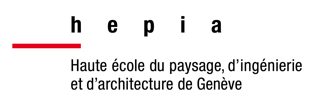
\includegraphics[scale=2]{imgs/hepia}
\end{center}

\vspace{3cm}

\begin{center}
\begin{huge}
\textbf{Rapport}
\end{huge}
\end{center}

\begin{center}
\begin{large}
Minix File system
\end{large}
\end{center}

% Trait de separation
\newcommand{\lineunder}{\color{bleuClair}\hrulefill\\\color{black}}
\lineunder

\begin{center}
\begin{large}
ITI 2\up{ème} soir \\
2014 / 2015
\end{large}
\end{center}

\vspace{3cm}
\centerline{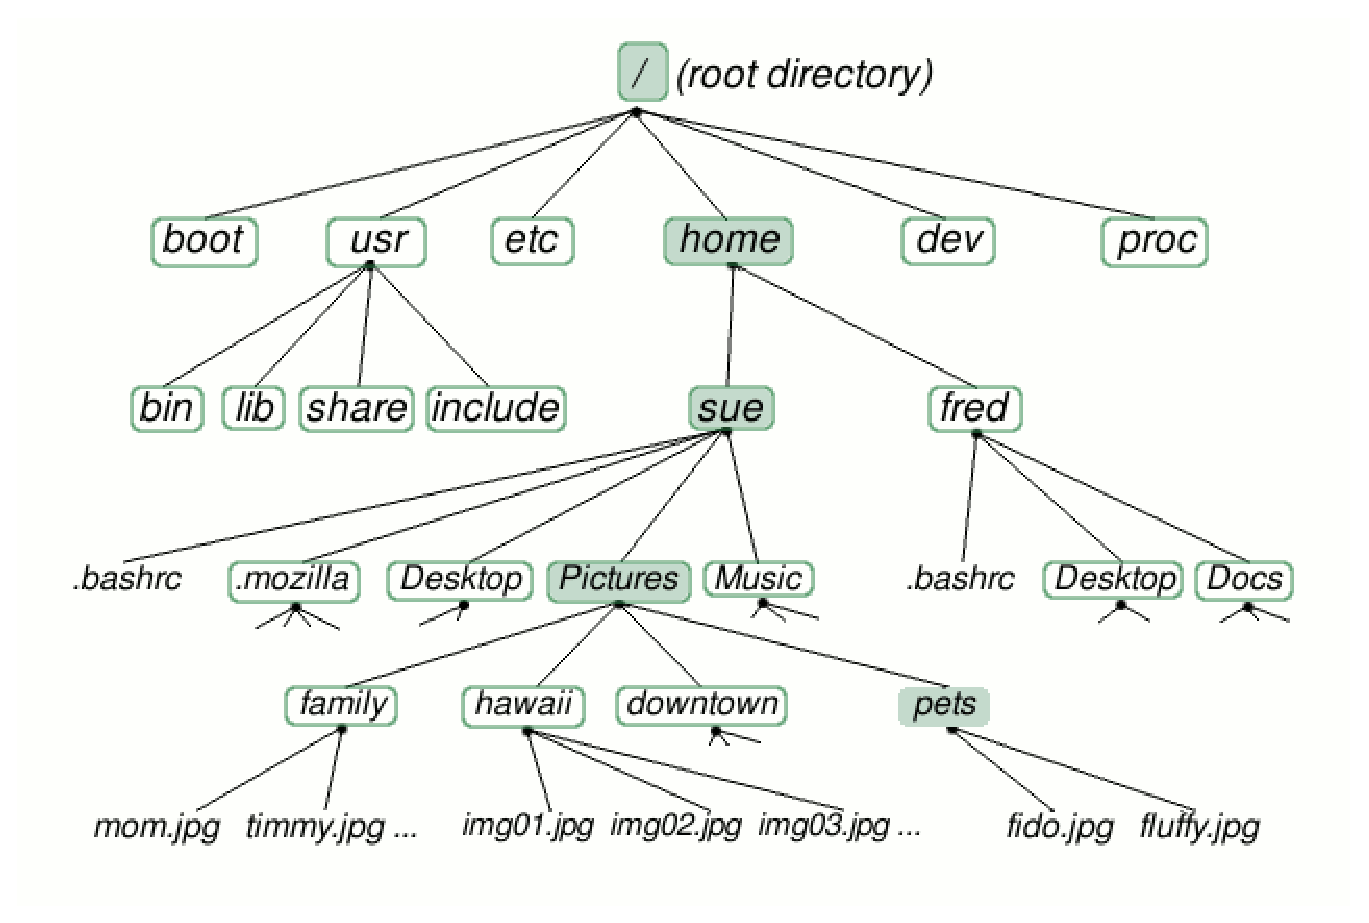
\includegraphics[scale=0.52]{imgs/illustration_FS}}
\vspace{2cm}

\begin{center}
%\begin{large}
\textbf{Sebastien Chassot} \\ Juin 2015
%\end{large}
\end{center}

\thispagestyle{empty} % enleve les entetes et pide de page de la page de titre

% table des matières
\newpage % nouvelle page
\tableofcontents % table des matières
\listoffigures
\listoftables
\newpage % nouvelle page

%\chapter*{Mini Bash}


\section{Introduction}

\vspace{1cm}
Le but de ce travail est d'implémenter un système MinixFS V1 en python en proposant une API standard et de modifier un fichier formaté en minixfs via cet interface.\\

Dans un deuxième temps, les modifications seront faites à travers le réseau. Un programme de test simple écrit en python utilise l'API mais les lectures/écritures sont faite par un server de blocs. Le server (écrit en C) modifiera le fichier selon les commandes reçues au travers d'une sockets AF\_INET. On réutilisera le travail fait en python et son API mais les blocs seront transmis au server selon un protocole relativement simple.

\vspace{2cm}

\begin{figure}[H]
\begin{center}
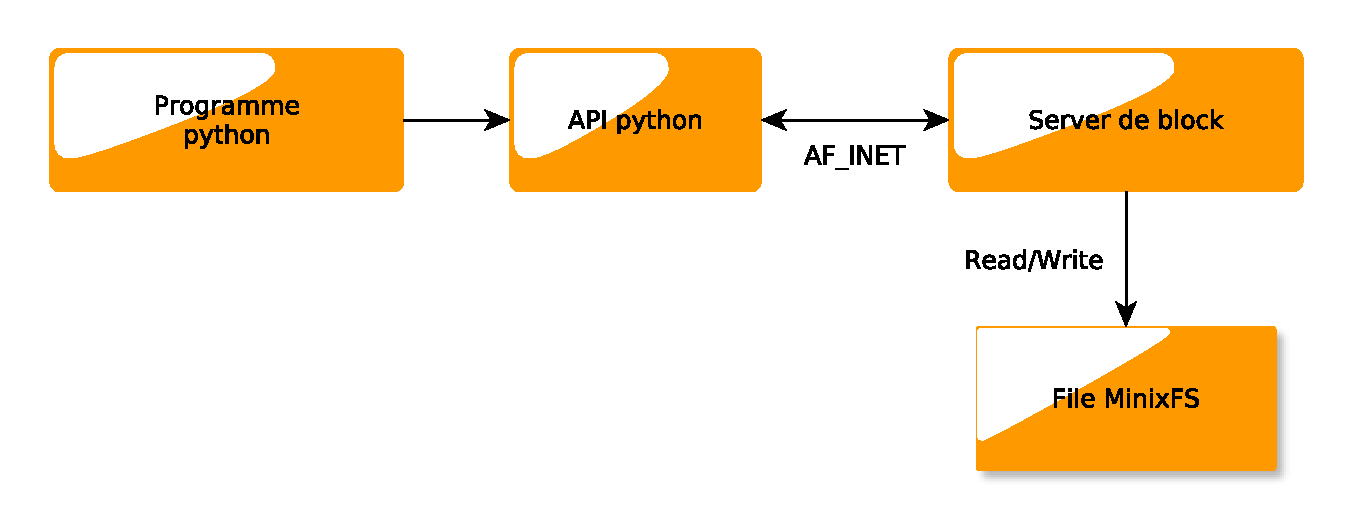
\includegraphics[scale=.6]{imgs/schema_client_server}
\caption{Principe de fonctionnement}
\label{fig:Architecture client server}
\end{center}
\end{figure}


Un seul client est traité à la fois ce qui évite les problèmes d'accès concurrent - traité dans d'autres cours. Le principe est simple; le client fait une requête, le server y répond.\\

\pagebreak

\section{Exécution du programme}

Toutes les commandes peuvent être lancées avec make.\\

Le projet est hébergé sur \url{https://github.com/selinux/tp-minixfs}

\begin{lstlisting}[language=bash,caption={lancer le server}]

pour les tests en local

	$ make test1
ou
	$ make test2
	
pour lancer la doc
	$ make doc

	$ ./server
	Usage : ./server <port> <file>
	
	
pour lancer le server avec make
	$ make server && make run

ou avec strace
	$ make server && make run_debug
	
dans un autre terminal
	$ make test_server

\end{lstlisting}

\pagebreak

\section{Implémentation python}

L'API implémentée est une version simplifiée d'un système de fichiers actuelle. On y retrouve les même méthodes et le fonctionnement global est le même.\\

\subsection{brève description de l'API}


\begin{description}
\item[ialloc()] \hfill \\
	alloue le premier inode de libre - puisqu'il contient peut-être d'ancienne donnée, il est remplacé par un nouvel inode vierge.
\item[ifree(inodenum)] \hfill \\
	change l'état de l'inode à \emph{libre} dans la bitmap des inodes. Cet inode sera donc libre pour une nouvelle allocation.
\item[balloc()] \hfill \\
	recherche et renvoie le premier block libre dans la bitmap des data block
\item[bfree(blocknum)] \hfill \\
	change l'état du data block à libre dans la bitmap (libre pour une future utilisation)
\item[bmap(inode, blk)] \hfill \\
	fait la transformation entre un numéro de block relatif et la position effective de ce block sur le disque
\item[lookup\_entry()] \hfill \\
	recherche une entrée dans un dossier et retourne l'inode de ce fichier
\item[namei(path)] \hfill \\
	Recherche en partant de la racine et en suivant l'arborescence jusqu'à trouver le fichier et renvoie son numéro d'inode
\item[ialloc\_bloc(inode, block)] \hfill \\
	Recherche un block de libre sur le disque et place 
\item[add\_entry(dinode, name, new\_inode\_number)] \hfill \\
	Ajoute une entrée dans un dossier
\end{description}


\subsection{Complément sur certaines méthodes}

\subsubsection*{bmap()}

Il y a un problème avec le test unitaire numéro 8. Si \emph{bmap()} vérifie la taille du fichier (valeur de l'inode). Le test echoue en effet, les 3 zones de l'inode sont testées. Une boucle va de 0 à 6 (direct), une autre de 7 à 518 (indirect) et la troisième va de 519 à 1024 (dbl\_indirect) or la taille du fichier est de 659'384 octets et occupe donc 644 blocks. Pour passer le test, il faut soit tester de 0 à 643, soit commenter les lignes suivantes.\\


\begin{lstlisting}[language=python, caption=test inode\_size in bmap]
        size = inode.i_size

        # the data block (>firstdatazone) must fit the inode size
        if self.is_file(inode) or self.is_link(inode):
            if blk > int(size / self.disk.blksize):
                raise MinixfsException('Error block is out of file boundary')
\end{lstlisting}

Dans le test b, \emph{ialloc\_bloc()} ajoute deux blocks sans modifier la taille ce qui fait échouer le test également.\\

\subsubsection*{lookup\_entry()}

Cette fonction va parcourir tous le dinode et créer un dictionnaire inode;nom\_fichier. À la fin, on retourne simplement l'entrée du dictionnaire associée au nom (le numéro d'inode). Cette solution est lourde puisqu'un dictionnaire est créé à chaque appel. C'était juste pour tester les fonctionnalités de python mais il serait bien plus efficace de faire un break dès que l'entrée est trouvée.\\


\subsubsection*{del\_entry()}

Avant de supprimer une entrée, il est préférable de tester s'il s'agit bien d'un dossier (et pas un fichier). Vérifier avec lookup\_entry() que le fichier existe bien dans le dossier.\\

Il faut également vérifier que le lien soit à 1, sinon il faut simplement décrémenter les liens mais garder l'inode (un autre fichier pointe dessus).\\

Une fois une entrée supprimée, le bloc est comparée à un bloc vide et supprimé s'il  n'est plus nécessaire.\\

\begin{lstlisting}[language=python, caption=test after del\_entry()]
            # after deleting entry, if dir_content is empty free the empty data bloc
            if dir_content == "".ljust(BLOCK_SIZE, '\x00'):
                self.bfree(dir_block)
\end{lstlisting}


\subsubsection*{ialloc\_bloc()}

Cette fonction attribue un block à n'importe quel position - dans un nouvel inode, on peut vouloir commencer par écrire le block \emph{2452} (dans la zone doublement indirect). Si le block doublement indirect indirect n'existe pas, il faut le créer, mettre l'adresse du nouveau bloc du fichier dedans et placer l'adresse du bloc dbl\_indirect dans le blocs dbl\_indirect.\\

Plus généralement, en allouant un bloc il faut pouvoir le faire quel que soit sa position.\\


\subsection{Logs et exceptions}

Dans tous le code du client, les erreurs lèvent une exception qui log une erreur \emph{log.error()} et l'affiche.\\

Dans le reste du programme, deux niveaux de log sont utilisé \emph{log.info()} et \emph{log.debug()}. Il suffit de changer \emph{log.basicConfig()} de \emph{level=log.INFO} à  \emph{level=log.DEBUG}.\\

Il y a aussi moyen de sortir les logs dans un fichier.\\


\begin{lstlisting}[language=python, caption=initialisation logs et exception MinixfsError()]
import logging as log

log.basicConfig(format='%(levelname)s:%(message)s', level=log.INFO)
#LOG_FILENAME = 'minixfs_tester.log'
#log.basicConfig(filename=LOG_FILENAME,level=log.DEBUG)

class MinixfsException(Exception):
    """ Class minixfs exceptions  """

    def __init__(self, message):
        super(MyBaseException, self).__init__(message)
        log.error(message)
        
        
\end{lstlisting}


\vspace{1cm}

\section{Le serveur de blocs}


\subsection{la problématique de la connexion}

Détecter la déconnexion d'un client est trivial (read() renvoit \emph{0}) mais comment réagir ? Le server en cas de déconnexion libère la mémoire et attend de nouveaux clients.\\

\subsection{Principe de fonctionnement du server}

La communication est bidirectionnelle mais le client initie toujours la communication. Le server ne fait que répondre aux requêtes.\\

Un client se connecte et le server accept() la connexion puis rentre dans une boucle - on aurait également pu faire un fork ou lancer un thread pour traiter le client.\\

Tant que le client ne se déconnecte pas, le server bloc sur le premier read et attend une requête.\\

Le server tourne dans une boucle infinie (le code suivant la boucle est inaccessible dans l'état actuel). Puis rentre dans une boucle (traitement du client) qui fait successivement :\\

\begin{center}
\begin{table}[H]
\begin{tabular}{| c | c |}
\hline
\multicolumn{2}{| c |}{lecture header requête (20 octets)}\\
\hline \hline
\textbf{read()} & \textbf{write()}\\
\hline \hline
lecture disque selon demande client & Lecture payload client\\
\hline
écriture header réponse (12 octets )& écriture payload sur le disque\\
\hline
écrit le payload réponse & écrire header réponse au client (12 octets)\\
\hline
\end{tabular}
\caption{Ordre lecture/écriture}
\label{succession lecture/écriture}
\end{table}
\end{center}

À chaque lecture ou écriture, si le client se déconnecte, le server revient à accept().\\

\begin{figure}[H]
\begin{center}
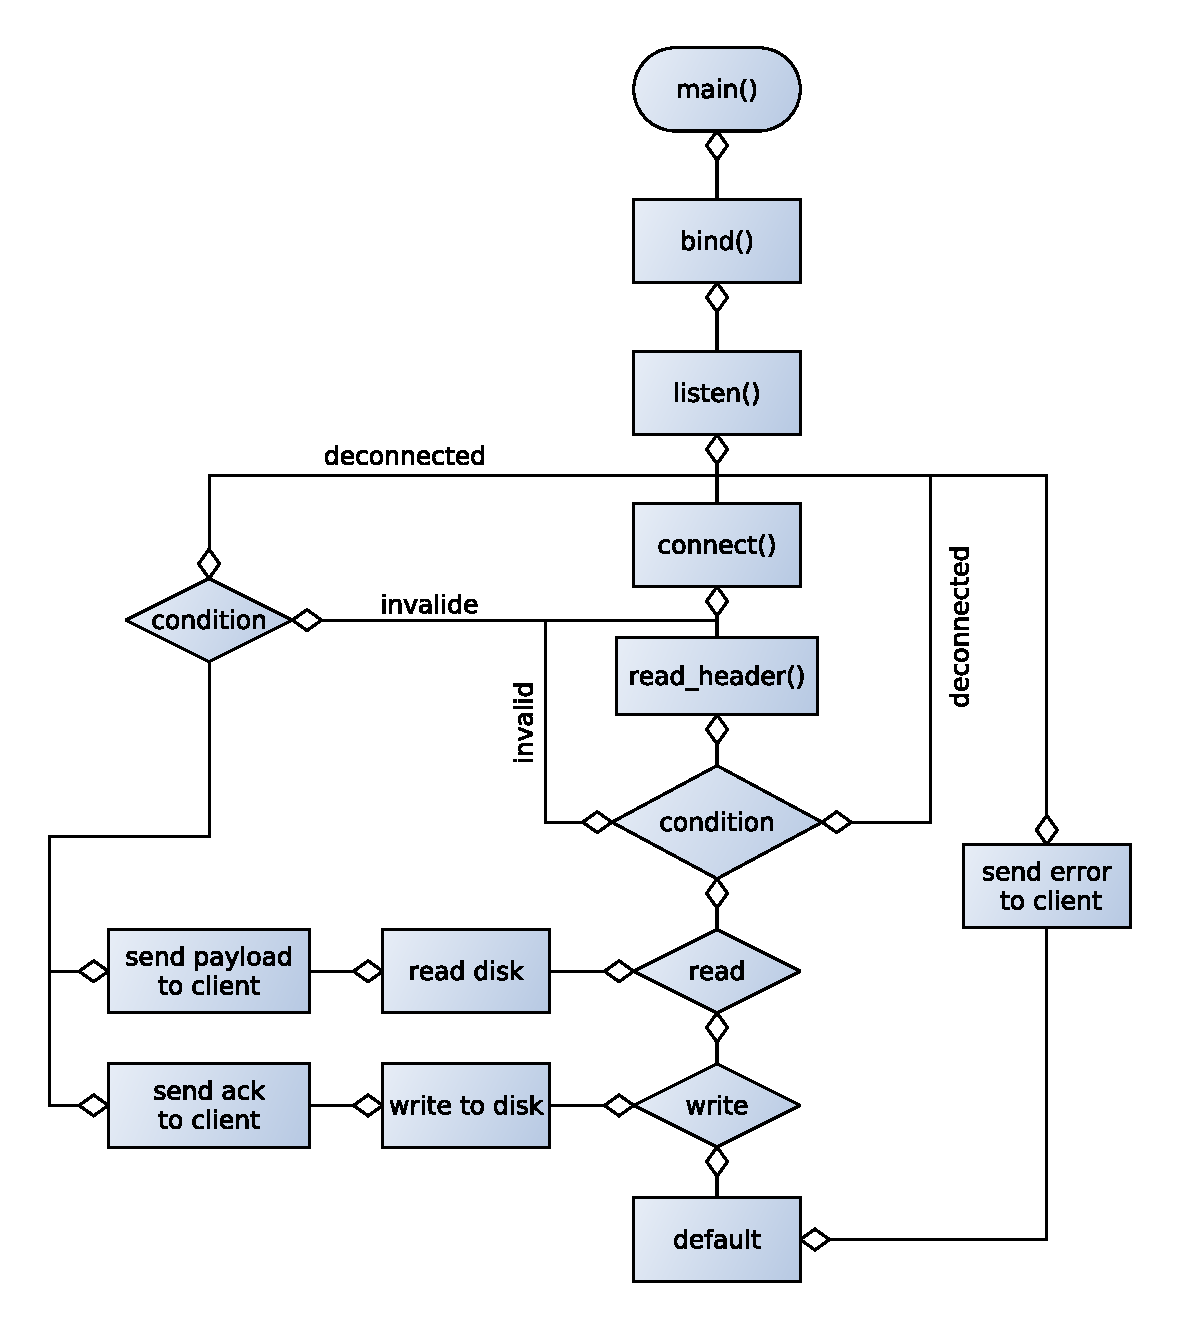
\includegraphics[scale=.6]{imgs/schema_server}
\caption{Principe de fonctionnement du server}
\label{fig:Architecture server}
\end{center}
\end{figure}

\subsection{Problème de sécurité}

C'est cette solution qui a été mise en place (dans une boucle infinie) mais elle ne permet pas de se protéger d'un client malveillant. Si un client ne respecte pas le protocole, le server peut se retrouver bloqué. Si un client annonce un payload d'une certaine longueur mais envoit d'autres données, il décale le flux et la communication serait désynchronisée laissant le server bloqué sur un read().\\


\subsection*{Solutions envisagées}

Une des solutions les plus simple serait de traiter les demandes l'une après l'autre; le client se connecte, envoie une requête, reçoit la réponse et se déconnecte. Le server fait la même chose; attend sur \emph{accept()} qu'un client se connecte puis traite la requête et y répond et se déconnecte.\\

Cette solution est simple, permet de mieux maîtriser la synchronisation  client/server mais est couteuse en connexions.\\


Une alternative possible est d'ajouter au protocole une requête (un message) de déconnexion qui synchronise le client et le server. On ajoute de la complexité au protocole.\\

Une autre serait de faire une machine d'état afin de s'assurer de l'état dans lequel est le client et le server et le passage entre chaque état. Si un problème arrive, revenir dans un état connu.


\section{Conclusion}

L'API python fonctionne bien et passe tous les tests unitaires. Il ne manquerait plus maintenant qu'à ajouter les appels systèmes en user space pour qu'il soit fonctionnel.\\

Le server de bloc fonctionne bien également et passe tous les tests mais est assez sensible à un client qui ne respecterait pas le protocole.\\



%\begin{lstlisting}[language=C, caption=pseudo code del\_entry()]
%struct timeval tv;
%fd_set readfds;
%int state;
%
%FD_ZERO(&readfds);
%
%tv.tv_sec = 5;
%tv.tv_usec = 0;
%
%client = accept(s, (struct sockaddr *) &addr_client, (socklen_t *) &s_len);
%
%FD_SET(client, &readfds);
%
%boucle {
%
%	state = select(n, &readfds, NULL, NULL, &tv);
%	
%	if(FD_ISSET(client, &readfds))
%		read_socket();
%	else
%		continue;
%
%...
%
%}
%\end{lstlisting}


%\section{Annexes}
%
%\subsection*{ialloc()}
%
%\begin{lstlisting}[language=C, caption=pseudo code ialloc()()]
%ialloc(){
%
%	recherche premier libre dans inode_map
%	
%	si not trouve:
%		raise error plus aucun inode de libre
%	
%	inode trouve = occupe
%	del ancien inode
%	new inode
%	
%	return numero inode
%}
%\end{lstlisting}
%
%\subsection*{ifree(inode)}
%
%\begin{lstlisting}[language=C, caption=pseudo code ifree()()]
%ifree( inode ){
%
%	inode = libre
%	return est-ce que inode est libre?
%}
%\end{lstlisting}
%
%\subsection*{balloc()}
%
%\begin{lstlisting}[language=C, caption=pseudo code balloc()()]
%balloc( ){
%
%	recherche premier block dans block map
%	si non trouver:
%		raise error plus de place sur disk
%	
%	block = occuper
%
%	return numero de block
%}
%\end{lstlisting}
%
%\subsection*{bfree(blocknum)}
%
%\begin{lstlisting}[language=C, caption=pseudo code bfree()()]
%bfree( data block ){
%
%	data block = libre
%	return est-ce que data block est libre?
%}
%\end{lstlisting}
%
%\subsection*{bmap()}
%
%\begin{lstlisting}[language=C, caption=pseudo code bmap()()]
%bmap( numero inode, position relative block ){
%
%	si block < 7:
%		return position du nieme block direct
%		
%	block -= 7
%	si block < nombre inode par block:
%		return position du nieme block de indirect
%	
%	block -= nombre inode par block
%	si block < (nombre inode par block)^2:
%		adresse	data block = block / nombre inode par block
%		position block = block mod nombre inode par block
%		
%		return numero block a adresse.posistion
%		
%	sinon:
%		raise error depassement de capacite
%}
%\end{lstlisting}
%
%\subsection*{add\_entry()}
%
%\begin{lstlisting}[language=C, caption=pseudo code add\_entry()]
%add_entry(inode dossier, nom fichier a inserer, inode du nouveau fichier){
%	si nom de fichier non conforme;
%		raise error
%	si nom de fichier existe deja dans dossier:
%		raise error
%		
%	tant que not done:
%		prendre block dossier:
%			si place libre:
%				inserer inode et nom
%				changer taille dossier
%				done
%
%			sinon:
%				si not next block:
%					creer nouveau block
%					si plus possible creer:
%						break
%						
%	si done:
%		valider modification sur disk
%	sinon:
%		raise error plus de place
%}
%\end{lstlisting}
%
%
%\subsection*{del\_entry()}
%
%\begin{lstlisting}[language=C, caption=pseudo code del\_entry()]
%del_entry(inode dossier, nom fichier a supprimer){
%	rechercher_entree;
%	si (non trouve)
%		raise error;
%
%	tant que block dossier:
%		rechercher entree dans block dossier
%			trouver:
%				si plusieurs liens: reduire
%				sinon: effacer inode fichier
%			
%				enlever entree du block dossier;
%				reduire taille dossier
%				si dernier fichier du block dossier supprimer block inutile;
%	
%	valider modification sur disk;
%}
%\end{lstlisting}


\end{document} 